\subsection{Plan Selector}

% [ERIC/KARTHIK - 1 pg]

% Decision logic, tabular spec and evolution, APT synth and proof \\

% might want to cite Alessandro's recent APT/ATJ/ATC papers?

A critical component of the RTA architecture is the Plan Selector, which selects the flight
plan to be used based on formally verified decision logic. This decision logic specifies the rules
that determine whether the LEC flight plan or the Backup Avoidance flight plan (BAF) should
be selected based on the results received from the RWC Assessment component. The
decision logic is specified in a tabular format, shown in Figure~\ref{fig:selection-logic}.
After running the logic, the Plan Selector sends its decision to the
aircraft Plan Switch.

When a flight plan assessment is received, it is evaluated based on five
variables, including the RWC metrics:  plan validity (whether a plan has been received), plan
safety, whether the time of closest point of approach (tCPA) is greater than
179 seconds (the end of the planning horizon), comparison of the predicted miss
distance (pmd) between the intruder and own-ship, and whether three seconds has elapsed since the
receipt of the first plan.

If only one plan has been received by the three second timeout, we select (publish)
that plan by default.
If we receive two plans and only one is safe, we select the safe plan.
If neither plan is safe, we select the one with the larger predicted miss distance.
If both plans are safe, the LEC plan is usually selected.  However, there is some
additional tie-breaking logic.
If tCPA is beyond the planning horizon for one of the plan, this means that we don't really know what
its true CPA is so we select the other plan.
If tCPA is beyond the planning horizon for both plans, we fall back to selecting the plan with
the greater predicted miss distance.

Different selection logic could be specified depending on vehicle and program requirements,
and indeed our specification evolved over the course of the project.  However, the
formal synthesis approach (described in the next section) ensures that we can
quickly regenerate a correct implementation of the specification.

%not valid, we deem it unfit for publication.  If a plan is valid, and we've yet
%to receive the other plan after 3 seconds, we go ahead and publish the plan we
%received.  Otherwise, we've received two valid plans.  If exactly one of them
%is safe, we publish it.  If neither plan is safe, we publish the one with the
%larger predicted miss distance.
%Otherwise, both plans are safe, so we consider
%whether their times of closest approach are beyond the 179 second limit.  If
%exactly one plan's tCPA is beyond the limit, we choose the other plan.  If
%neither is beyond the limit, we chose the LEC plan.  Otherwise, both plans'
%tCPA is beyond the 179 second limit.  In that case, we choose the plan with the
%larger predicted miss distance.  See Figure~\ref{fig:selection-logic} for the
%full decision table.

\begin{figure*}
	\centering
	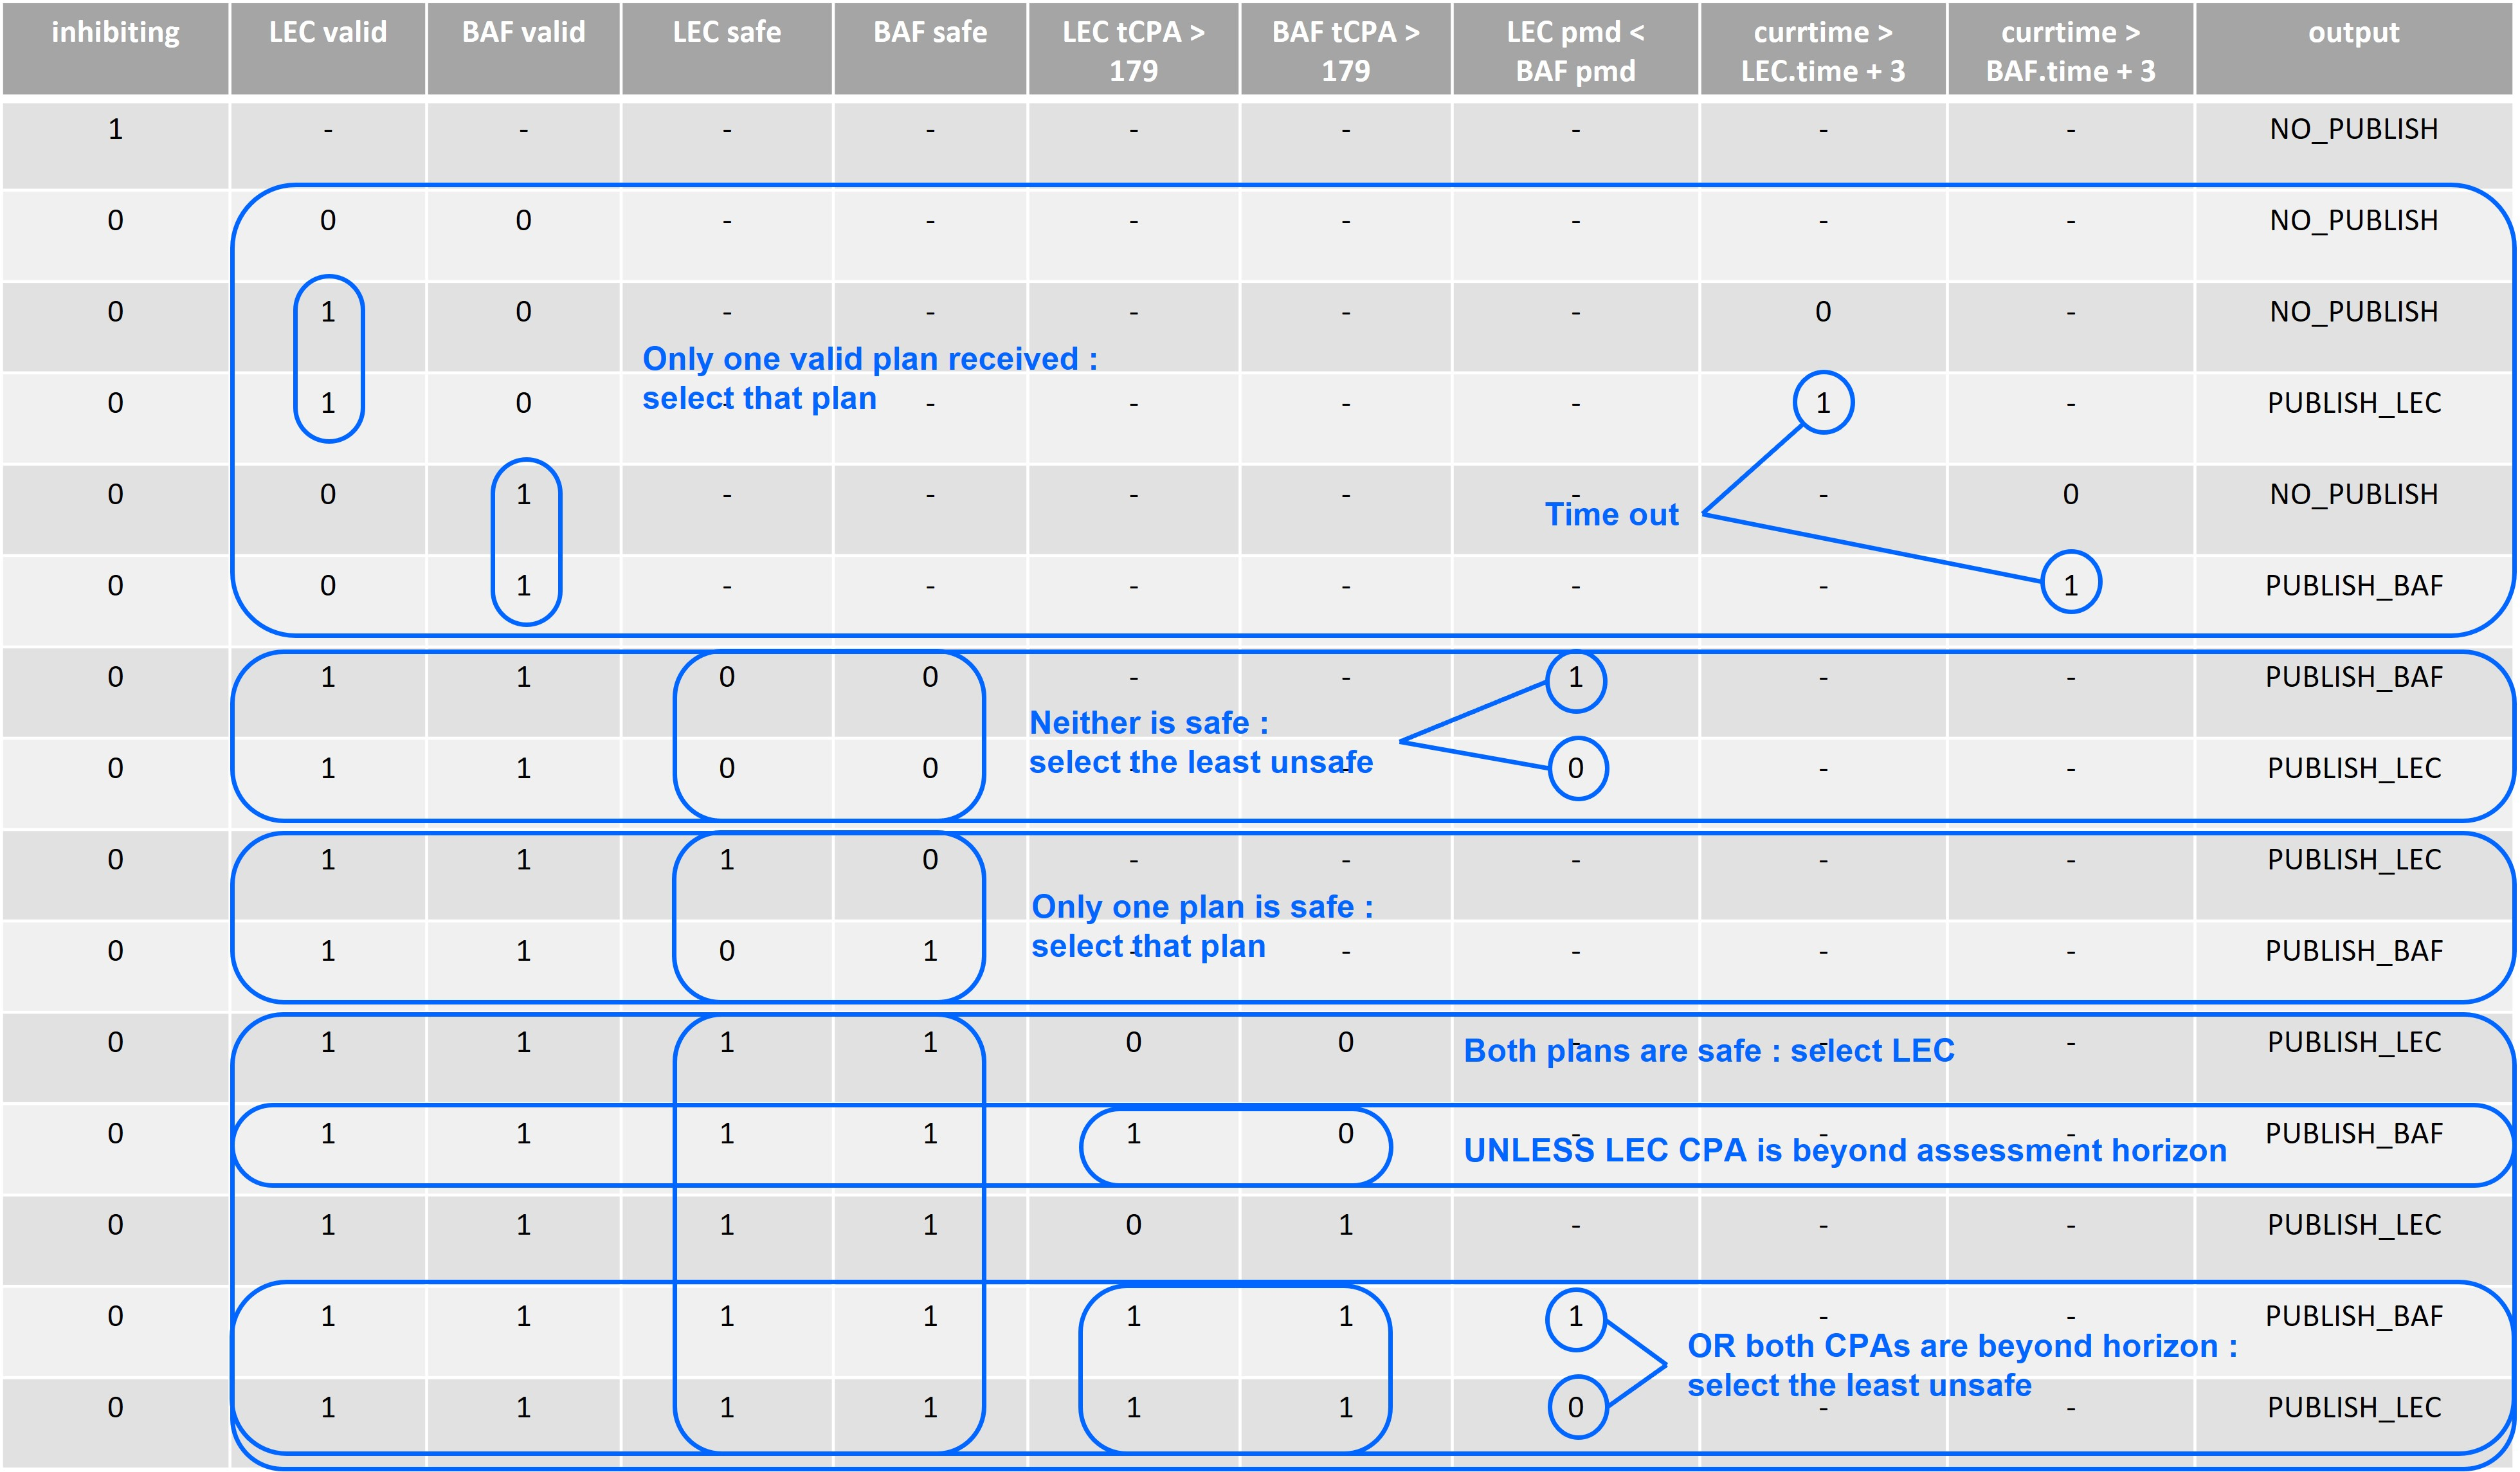
\includegraphics[width=\textwidth]{figures/selection-logic.jpg}
	\caption{Plan Selection logic specification (hyphens match either 0 or 1)}
	\label{fig:selection-logic}
\end{figure*}
